\newcounter{english}
\documentclass{article}

% packages
\usepackage{amsmath, amsthm, thmtools, amsfonts, amssymb, luacode, catchfile, tikzducks, hyperref, ifthen}
\ifcsname c@kobocompile\endcsname
	\usepackage[a5paper, total={1072pt, 1448pt}, margin=10pt, includeheadfoot]{geometry} % set page margins
\else
	\usepackage[a4paper, margin=50pt, includeheadfoot]{geometry}
\fi
\usepackage[shortlabels]{enumitem}
\usepackage[skip=3pt, indent=0pt]{parskip}

% language
\usepackage[bidi=basic, layout=tabular, provide=*]{babel}
\ifcsname c@english\endcsname
	\babelprovide[main, import]{english}
\else
	\babelprovide[main, import]{hebrew}
	\babelprovide{rl}
\fi
%\babelfont{rm}{Libertinus Serif}
\babelfont{rm}[Renderer=Harfbuzz]{Libertinus Serif}
\babelfont{sf}{Libertinus Sans}
\babelfont{tt}{Libertinus Mono}

% style
\AddToHook{cmd/section/before}{\clearpage}	% Add line break before section
\linespread{1.3}
\setcounter{secnumdepth}{0}		% Remove default number tags from sections, this won't do well with theorems
\AtBeginDocument{\setlength{\belowdisplayskip}{3pt}}
\AtBeginDocument{\setlength{\abovedisplayskip}{3pt}}
\graphicspath{ {../images/} }

% operators
\DeclareMathOperator\cis{cis}
\DeclareMathOperator\Sp{Sp}
\DeclareMathOperator\tr{tr}
\DeclareMathOperator\im{Im}
\DeclareMathOperator\re{Re}
\DeclareMathOperator\diag{diag}
\DeclareMathOperator*\lowlim{\underline{lim}}
\DeclareMathOperator*\uplim{\overline{lim}}
\DeclareMathOperator\rng{rng}
\DeclareMathOperator\Sym{Sym}
\DeclareMathOperator\Arg{Arg}
\DeclareMathOperator\Log{Log}
\DeclareMathOperator\dom{dom}
\DeclareMathOperator\supp{Supp}
\DeclareMathOperator\var{Var}
\DeclareMathOperator\cov{Cov}

% commands
%\renewcommand\qedsymbol{\textbf{מש''ל}}
%\renewcommand\qedsymbol{\fbox{\emoji{lizard}}}
\newcommand{\Aa}[0]{\mathcal{A}}
\newcommand{\Bb}[0]{\mathcal{B}}
\newcommand{\CC}[0]{\mathbb{C}}
\newcommand{\Cc}[0]{\mathcal{C}}
\newcommand{\EE}[0]{\mathbb{E}}
\newcommand{\FF}[0]{\mathbb{F}}
\newcommand{\Ff}[0]{\mathcal{F}}
\newcommand{\Ii}[0]{\mathcal{I}}
\newcommand{\Gg}[0]{\mathcal{G}}
\newcommand{\Ll}[0]{\mathcal{L}}
\newcommand{\Mm}[0]{\mathcal{M}}
\newcommand{\NN}[0]{\mathbb{N}}
\newcommand{\Nn}[0]{\mathcal{N}}
\newcommand{\PP}[0]{\mathbb{P}}
\newcommand{\Pp}[0]{\mathcal{P}}
\newcommand{\QQ}[0]{\mathbb{Q}}
\newcommand{\RR}[0]{\mathbb{R}}
\newcommand{\Rr}[0]{\mathcal{R}}
\newcommand{\Ss}[0]{\mathcal{S}}
\newcommand{\TT}[0]{\mathbb{T}}
\newcommand{\Uu}[0]{\mathcal{U}}
\newcommand{\Vv}[0]{\mathcal{V}}
\newcommand{\Ww}[0]{\mathcal{W}}
\newcommand{\ZZ}[0]{\mathbb{Z}}
\newcommand{\acts}[0]{\circlearrowright}
\newcommand{\explain}[2] {
	\begin{flalign*}
		 && \text{#2} && \text{#1}
	\end{flalign*}
}
\newcommand{\maketitleprint}[0]{ \begin{center}
	%\begin{tikzpicture}[scale=3]
	%	\duck[graduate=gray!20!black, tassel=red!70!black]
	%\end{tikzpicture}	
	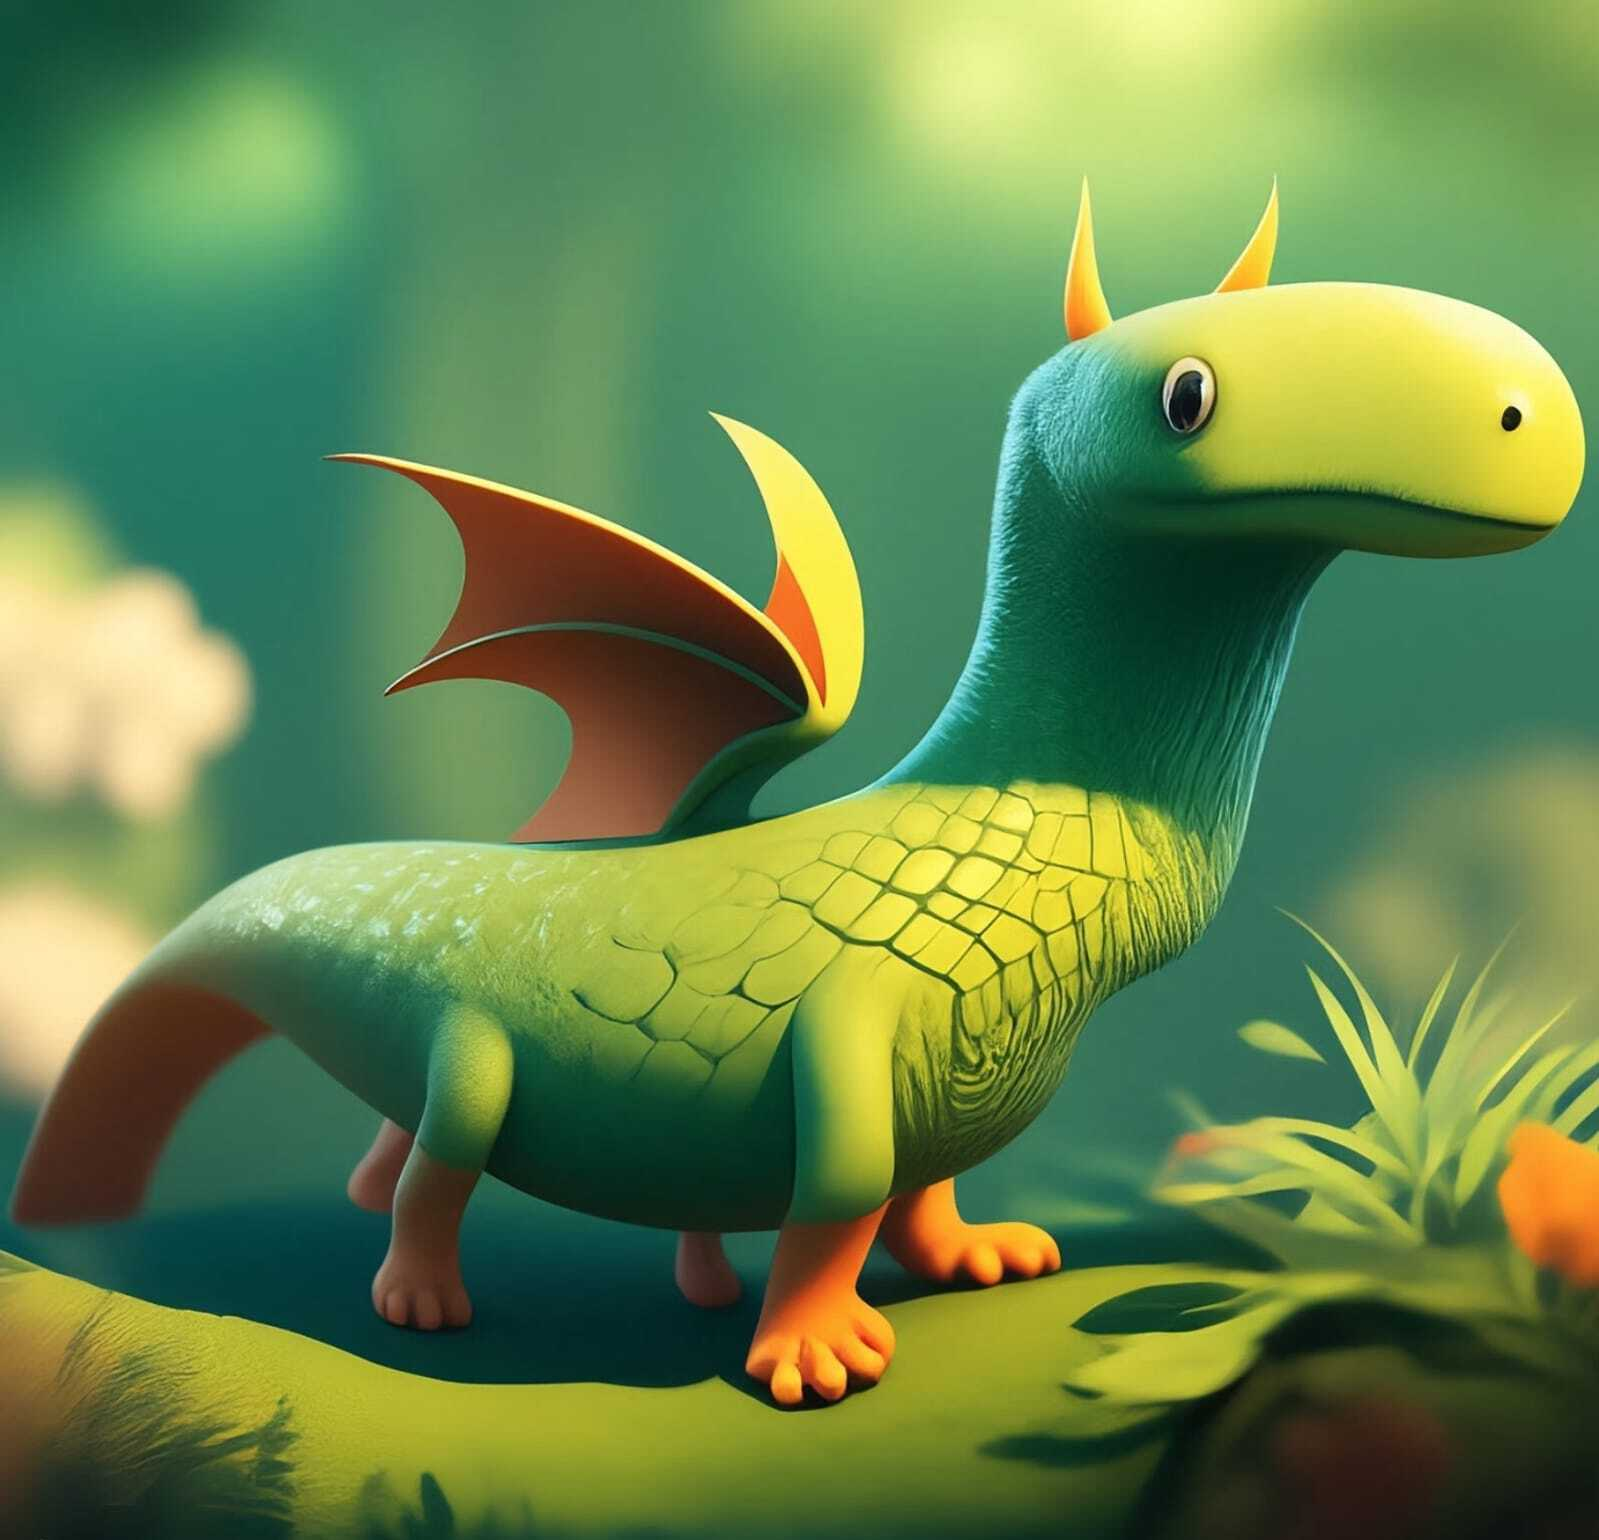
\includegraphics[width=6cm]{cover}
\end{center}
}

% theorem commands
\newtheoremstyle{c_remark}
	{}	% Space above
	{}	% Space below
	{}% Body font
	{}	% Indent amount
	{\bfseries}	% Theorem head font
	{}	% Punctuation after theorem head
	{.5em}	% Space after theorem head
	{\thmname{#1}\thmnumber{ #2}\thmnote{ \normalfont{\text{(#3)}}}}	% head content
\newtheoremstyle{c_definition}
	{3pt}	% Space above
	{3pt}	% Space below
	{}% Body font
	{}	% Indent amount
	{\bfseries}	% Theorem head font
	{}	% Punctuation after theorem head
	{.5em}	% Space after theorem head
	{\thmname{#1}\thmnumber{ #2}\thmnote{ \normalfont{\text{(#3)}}}}	% head content
\newtheoremstyle{c_plain}
	{3pt}	% Space above
	{3pt}	% Space below
	{\itshape}% Body font
	{}	% Indent amount
	{\bfseries}	% Theorem head font
	{}	% Punctuation after theorem head
	{.5em}	% Space after theorem head
	{\thmname{#1}\thmnumber{ #2}\thmnote{ \text{(#3)}}}	% head content

\ifcsname c@english\endcsname
	\theoremstyle{plain}
	\newtheorem{theorem}{Theorem}[section]
	\newtheorem{lemma}[theorem]{Lemma}
	\newtheorem{proposition}[theorem]{Proposition}
	\newtheorem*{proposition*}{Proposition}
	%\newtheorem{corollary}[theorem]{אין חלופה עברית}

	\theoremstyle{definition}
	\newtheorem{definition}[theorem]{Definition}
	\newtheorem*{definition*}{Definition}
	\newtheorem{example}{Example}[section]
	\newtheorem{exercise}{Exercise}[section]

	\theoremstyle{remark}
	\newtheorem*{remark}{Remark}
	\newtheorem*{solution}{Solution}
	\newtheorem{conclusion}[theorem]{Conclusion}
	\newtheorem{notation}[theorem]{Notation}
\else
	\theoremstyle{c_plain}
	\newtheorem{theorem}{משפט}[section]
	\newtheorem{lemma}[theorem]{למה}
	\newtheorem{proposition}[theorem]{טענה}
	\newtheorem*{proposition*}{טענה}
	%\newtheorem{corollary}[theorem]{אין חלופה עברית}

	\theoremstyle{c_definition}
	\newtheorem{definition}[theorem]{הגדרה}
	\newtheorem*{definition*}{הגדרה}
	\newtheorem{example}{דוגמה}[section]
	\newtheorem{exercise}{תרגיל}[section]

	\theoremstyle{c_remark}
	\newtheorem*{remark}{הערה}
	\newtheorem*{solution}{פתרון}
	\newtheorem{conclusion}[theorem]{מסקנה}
	\newtheorem{notation}[theorem]{סימון}
\fi

% Questions related commands
\newcounter{question}
\setcounter{question}{1}
\newcounter{sub_question}
\setcounter{sub_question}{1}

\ifcsname c@english\endcsname
	\newcommand{\question}[1][0]{
		\ifthenelse{#1 = 0}{}{\setcounter{question}{#1}}
		\section{Question \arabic{question}}
		\addtocounter{question}{1}
		\setcounter{sub_question}{1}
	}

	\newcommand{\subquestion}[1][0]{
		\ifthenelse{#1 = 0}{}{\setcounter{sub_question}{#1}}
		\subsection{Part \alph{sub_question}}
		\addtocounter{sub_question}{1}
	}
\else
	\newcommand{\question}[1][0]{
		\ifthenelse{#1 = 0}{}{\setcounter{question}{#1}}
		\section{שאלה \arabic{question}}
		\addtocounter{question}{1}
		\setcounter{sub_question}{1}
	}

	\newcommand{\subquestion}[1][0]{
		\ifthenelse{#1 = 0}{}{\setcounter{sub_question}{#1}}
		\subsection{סעיף \localecounter{letters.gershayim}{sub_question}}
		\addtocounter{sub_question}{1}
	}
\fi

% import lua and start of document
\directlua{common = require ('../common')}

\GetEnv{AUTHOR}

% headers
\author{\AUTHOR}
\date\today

\title{Exercise 8 Answer Sheet --- Axiomatic Set Theory, 80650}

\DeclareMathOperator{\crit}{crit}

\begin{document}
\maketitle
\maketitleprint{}

\question{}
\begin{definition}
	Let $X$ be a set. A tree $T$ is set such that,
	\begin{enumerate}
		\item For every $\eta \in T$, $\eta$ is a function from an ordinal $\alpha$ to $X$.
		\item If $\eta \in T$ and $\dom \eta = \alpha > \beta$ then $\eta \restriction \beta \in T$.
	\end{enumerate}
	If $X = 2$ then we say that $T$ is binary tree. \\
	The height of $T$ is the least ordinal $\alpha$ such that $\forall \eta \in T, \dom \eta < \alpha$.
	We define $\operatorname{Lev}(\eta) = \dom \eta$ (the level of $\eta$), and we denote $T_\alpha = \{\eta \in T \mid \operatorname{Lev}(\eta) = \alpha\}$.
	For $\eta, \eta' \in T$ we define $\eta \le_T \eta'$ if $\eta = \eta' \restriction \dom \eta$.
\end{definition}
\begin{definition}
	Let $\kappa$ be a regular cardinal, we say that a tree $T$ is a $\kappa$-tree if the height of $T$ is $\kappa$ and for every $\alpha < \kappa$, $|T_\alpha| < \kappa$.
\end{definition}
\begin{definition}
	Let $T$ be a tree of height $\alpha$.
	A function $b : \alpha \to X$ is a cofinal branch in $T$ if for every $\beta < \alpha$, $b \restriction \beta \in T$.
	We would also use the term cofinal branch for the set $\{ b \restriction \beta \mid \beta < \alpha \}$.
\end{definition}

Let $\kappa$ be an infinite regular cardinal.
Let $T$ be a binary $\kappa$-tree.

We will prove that there is $T' \subseteq T$ of height $\kappa$ such that for every $\alpha < \beta < \kappa$ and $x \in T'$ with $\operatorname{Lev}(x) = \alpha$,
there is $y \in T'$ with $\operatorname{Lev}(y) = \beta$ and $x \le_T y$.
\begin{proof}
	Let us define $T_0 = \{ x \in T \mid \forall \operatorname{Lev}(x) < \alpha < \kappa, \exists y \in T, y \in T_\alpha, x \le_T y \}$.
	If $T_0$ is a $\kappa$-tree then it satisfies the required property, then we will show it is indeed a tree of height $\kappa$.

	For every $x \in T_0$, $x \in T$, hence is a map from an ordinal to $X$.
	Assume $y \in T_0$, and let $x = y \restriction \beta$ for $\beta < \kappa$.
	For every $\beta < \gamma < \kappa$ there is $x \le_T y \le_T z$ such that the given property is satisfied.
	We assume $\alpha < \gamma < \beta$, then $y \restriction \gamma \in T_\gamma$ as $y \in T$.
	We can conclude $x \in T_0$, meaning $T_0$ satisfies definition, namely $T_0$ is a tree.

	We move to proving $T_0$ is of height $\kappa$.
	For certain $x \in T_0$ for every $\dom x < \alpha$ there is $y_\alpha \in T_0$ such that $\dom y_\alpha = \alpha$ for evert such ordinal, then $\sup_{\alpha < \kappa} y_\alpha = \kappa$ as intended.
	The claim is not about $T'$ being $\kappa$-tree (I hope), but we know that each level of $T_0$ must be bounded by the equivalent level in $T$, meaning it is bounded by $\kappa$.

	Lastly, we will check if $T_0$ in not empty, fulfilling our claims stated above.
	By the definition of $T$, if we select $\alpha = 0$, by the height of $T$ the statement is indeed true, indicating $\emptyset \in T_0$.

	We showed that there is such $T' = T_0$.
\end{proof}

\question{}
We will show that every binary $\omega$-tree has a cofinal branch.
\begin{proof}
	From the last question, we can assume $T' \subseteq T$ fulfills the property of arbitrary elements, then we will define recursively the function $b : \omega \to X$ by the following,
	\begin{enumerate}
		\item $b(0) = \eta(0)$, when $\eta$ is any branch $\in T$ (the root of ordered tree is unique).
		\item If $b \restriction n$ is already set, then $b(n) \in T_n$ such that $b(n - 1) \le_T b(n)$, there exists such in $T'$.
	\end{enumerate}
	The result is indeed $b : \omega \to X$ such that $b \restriction n \in T' \subseteq T$ for all $n < \omega$,
	meaning $b$ is cofinal branch of $T$ as desired.
\end{proof}

\question{}
We will prove that if there is some cardinal $\mu$ such that $\mu^+ < \kappa$ and $|T_\alpha| \le \mu$ for all $\alpha$, then $T$ has a cofinal branch.
\begin{proof}
	We assume such $\mu$ exists, as well without loss of generality the arbitrary height of branches is fulfilled.
	For each $x \in T$ such that $\alpha = \operatorname{Lev}(x)$, we let $\beta_x$ be the largest ordinal such that there is no other $y \in T_\alpha$ such that $y \restriction \beta_x = x \restriction \beta_x$.
	In other words, we get the highest level in which $x$ is the only continuation (as of branch) of some branch of that level.
	For each level $\alpha$ we define $f(\alpha) = \sup_{x \in T_\alpha} \beta_x$, $f$ mapping each level to the least level below it such that there is uniquely-extendable branch between the levels.
	Let $\dom f = S = \{ \alpha < \kappa \mid \mu^+ < \alpha \}$, then $S$ is stationary in $\kappa$, and $f : S \to \kappa$.
	By the definition, $f(\alpha) \le \alpha$.
	For every $x \in T_\alpha$ for $\alpha \in S$, we know that $|T_\alpha| \le \mu$, then there cannot be more than $\mu$ levels such that there are more continuations to the restricted branch of $x$,
	but $\operatorname{cf} \alpha \ge \mu^+$, meaning the set of such levels is bounded by $\beta < \mu^+$, in particular $\beta_x < \alpha$, then $f(\alpha) < \alpha$, namely $f$ is regressive.
	By Fodors lemma there is $T \subseteq S$ stationary in $\kappa$ such that $\forall x \in T, f(x) = \gamma$ for $\gamma < \kappa$.
	For some arbitrary $\alpha \in T$, let $x \in T_\alpha$ be a branch for which $\beta_x = \gamma$.
	For each $\alpha \in T$, we can conclude $\beta_x = \gamma$.
	$T$ is stationary therefore unbounded in $\kappa$, then for every $\delta < \kappa$, there is $\delta < \delta' \in T$.
	For this $\delta'$ there is a branch $x \le_T y \in T_{\delta'}$ by the arbitrary height claim, and $\beta_y = \gamma$ as well.
	We can define then $b : \kappa \to X$ by setting $b \restriction \delta = y$ for each $\delta < \kappa$, therefore $b$ is a cofinal branch of $T$.
\end{proof}

\question{}
Let us assume that there is a cardinal $\mu < \kappa$ and a function $f : T \to \mu$ such that for all $x, y \in T$, if $x <_T y$ then $f(x) \ne f(y)$. \\
We will prove that there is no cofinal branch in $T$.
\begin{proof}
	We assume by contradiction that $b : \kappa \to X$ is a cofinal branch of $T$.
	By transitivity of $<_T$ it follows that $f(b \restriction \alpha) \ne f(b \restriction \beta)$ for all $\alpha < \beta < \kappa$.
	We can deduce that for $X = f '' \{ b \restriction \alpha \mid \alpha < \kappa \}$, $|X| = \kappa$, in contradiction to $X \subseteq \rng f = \mu < \kappa$.
\end{proof}

\question{}
Let $\kappa$ be a measurable cardinal. \\
We will prove that every $\kappa$-tree has a cofinal branch.
\begin{proof}
	If $\kappa \le 2^{\aleph_0}$ then we already know that every $\kappa$-tree has cofinal branch.
	We assume that $2^{\aleph_0} < \kappa$, then the measure is $\kappa$-complete and we can assume that $\kappa$ is inaccessible (strong?).

	By the inaccessibility and $\kappa$ being regular we can deduce there is no mapping from $\alpha < \kappa$ to $|T_\alpha|$ such that $|T_\alpha| = \kappa$.
	Then there is an ordinal $\mu$, by the inaccessibility of $\kappa$, such that $|T_\alpha| \le \mu$ for all $\alpha < \kappa$.
	Then we can use the previous question to deduce that there is a cofinal branch in $T$.
\end{proof}

\end{document}
